\documentclass[a4paper, 14pt]{extarticle}

% Поля
%--------------------------------------
\usepackage{geometry}
\geometry{a4paper,tmargin=2cm,bmargin=2cm,lmargin=3cm,rmargin=1cm}
%--------------------------------------


%Russian-specific packages
%--------------------------------------
\usepackage[T2A]{fontenc}
\usepackage[utf8]{inputenc} 
\usepackage[english, main=russian]{babel}
%--------------------------------------

\usepackage{textcomp}

% Красная строка
%--------------------------------------
\usepackage{indentfirst}               
%--------------------------------------             


%Graphics
%--------------------------------------
\usepackage{graphicx}
\graphicspath{ {./images/} }
\usepackage{wrapfig}
%--------------------------------------

% Полуторный интервал
%--------------------------------------
\linespread{1.3}                    
%--------------------------------------

%Выравнивание и переносы
%--------------------------------------
% Избавляемся от переполнений
\sloppy
% Запрещаем разрыв страницы после первой строки абзаца
\clubpenalty=10000
% Запрещаем разрыв страницы после последней строки абзаца
\widowpenalty=10000
%--------------------------------------

%Списки
\usepackage{enumitem}

%Подписи
\usepackage{caption} 

%Гиперссылки
\usepackage{hyperref}

\hypersetup {
	unicode=true
}

%Рисунки
%--------------------------------------
\DeclareCaptionLabelSeparator*{emdash}{~--- }
\captionsetup[figure]{labelsep=emdash,font=onehalfspacing,position=bottom}
%--------------------------------------

\usepackage{tempora}
\usepackage{amsmath}
\usepackage{color}
\usepackage{listings}
\lstset{
  belowcaptionskip=1\baselineskip,
  breaklines=true,
  frame=L,
  xleftmargin=\parindent,
  language=Python,
  showstringspaces=false,
  basicstyle=\footnotesize\ttfamily,
  keywordstyle=\bfseries\color{blue},
  commentstyle=\itshape\color{purple},
  identifierstyle=\color{black},
  stringstyle=\color{red},
}

%--------------------------------------
%			НАЧАЛО ДОКУМЕНТА
%--------------------------------------

\begin{document}

%--------------------------------------
%			ТИТУЛЬНЫЙ ЛИСТ
%--------------------------------------
\begin{titlepage}
\thispagestyle{empty}
\newpage


%Шапка титульного листа
%--------------------------------------
\vspace*{-60pt}
\hspace{-65pt}
\begin{minipage}{0.3\textwidth}
\hspace*{-20pt}\centering

\includegraphics[width=\textwidth]{emblem}
\end{minipage}
\begin{minipage}{0.67\textwidth}\small \textbf{
\vspace*{-0.7ex}
\hspace*{-6pt}\centerline{Министерство науки и высшего образования Российской Федерации}
\vspace*{-0.7ex}
\centerline{Федеральное государственное бюджетное образовательное учреждение }
\vspace*{-0.7ex}
\centerline{высшего образования}
\vspace*{-0.7ex}
\centerline{<<Московский государственный технический университет}
\vspace*{-0.7ex}
\centerline{имени Н.Э. Баумана}
\vspace*{-0.7ex}
\centerline{(национальный исследовательский университет)>>}
\vspace*{-0.7ex}
\centerline{(МГТУ им. Н.Э. Баумана)}}
\end{minipage}
%--------------------------------------

%Полосы
%--------------------------------------
\vspace{-25pt}
\hspace{-35pt}\rule{\textwidth}{2.3pt}

\vspace*{-20.3pt}
\hspace{-35pt}\rule{\textwidth}{0.4pt}
%--------------------------------------

\vspace{1.5ex}
\hspace{-35pt} \noindent \small ФАКУЛЬТЕТ\hspace{80pt} <<Информатика и системы управления>>

\vspace*{-16pt}
\hspace{47pt}\rule{0.83\textwidth}{0.4pt}

\vspace{0.5ex}
\hspace{-35pt} \noindent \small КАФЕДРА\hspace{50pt} <<Прикладная Математика и информатика>>

\vspace*{-16pt}
\hspace{30pt}\rule{0.866\textwidth}{0.4pt}
  
\vspace{11em}

\begin{center}
\Large {\bf Лабораторная работа № 11} \\ 
\large {\bf по курсу <<Языки и методы программирования>>} \\ 
\large <<Разработка парсеров на языке Java>>
\end{center}\normalsize

\vspace{8em}


\begin{flushright}
  {Студент группы ИУ9-21Б Хромов М.А.\hspace*{15pt} \\
  \vspace{2ex}
  Преподаватель Посевин Д. П.\hspace*{15pt}}
\end{flushright}

\bigskip

\vfill
 

\begin{center}
\textsl{Москва 2025}
\end{center}
\end{titlepage}
%--------------------------------------
%		КОНЕЦ ТИТУЛЬНОГО ЛИСТА
%--------------------------------------

\renewcommand{\ttdefault}{pcr}

\setlength{\tabcolsep}{3pt}
\newpage


 

\section{Задание}\label{Sect::task}
\par
В ходе лабораторной работы нужно разработать программу, выполняющую
синтаксический анализ текста по одной из LL(1)-грамматик, БНФ которых приведены в
таблицах 1–6. Текст может содержать символы перевода строки.
В записи БНФ терминальные символы IDENT, NUMBER и STRING означают
идентификаторы, числа и строки, соответственно. Идентификатор – это последовательность
букв и цифр, начинающаяся с буквы. Число – это непустая последовательность десятичных
цифр. Строка – это обрамлённая кавычками произвольная последовательность символов, не
содержащая кавычек и символов перевода строки.
Программа должна выводить в стандартный поток вывода последовательность правил
грамматики, применение которых даёт левый вывод введённого из стандартного потока
ввода текста. Если вывод не может быть построен, программа должна выводить сообщение
«syntax error at (line, col)», где line и col – координаты ошибки в тексте.
\section{Индивидуальный вариант}\label{Sect::task}
\par
Реализовать БНФ для предложений таких, как: int *(*a[10][20])[5]
\section {Практическая реализация}
Исходный код программы представлен в листингах 1-4
\begin{figure}[!htb]
\begin{lstlisting}[language={},caption={класс},label={lst:code1}]
import java.util.ArrayList;
import java.util.List;

public class Parser {//список токенв из лексы
    private final List<Token> tokens;
    private int pos = 0;//текущ поз в списке
    private final List<String> rules = new ArrayList<>();//журнал разбора

    public Parser(List<Token> tokens) { //принимает список токенов
        this.tokens = tokens;
    }

    private Token sym() {
        if (pos >= tokens.size()) return new Token("EOF", "", -1, -1);
        return tokens.get(pos);
    }//возвращаем текущий токен, если вышел за границу - еоф

    private void next() {
        pos++;
    }
    //выбрасываю искл с коорд ошибки
    private void error(Token t) {
        throw new RuntimeException("syntax error at (" + t.line + ", " + t.col + ")");
    }

    public void parseDecl() {
        rules.add("<Decl> ::= <Type> <Ptr>"); //тип и указатель птр
        parseType();
        parsePtr();
        if (!sym().type.equals("EOF")) {//лишние символы
            error(sym());
        }
    }
    //int or float
    private void parseType() {
        Token t = sym();
        if (t.type.equals("IDENT") && (t.value.equals("int") || t.value.equals("float"))) {
            rules.add("<Type> ::= " + t.value);
            next();
        } else {
            error(t);
        }
    }
    //<Ptr> — может быть либо * <Ptr>, либо <Prim> <Dims>
    private void parsePtr() {
        Token t = sym();
        if (t.type.equals("*")) {
            rules.add("<Ptr> ::= * <Ptr>");
            next();
            parsePtr();
        } else {
            rules.add("<Ptr> ::= <Prim> <Dims>");
            parsePrim();
            parseDims();
        }
    }
    //<Prim> — либо IDENT, либо (<Ptr>)
    private void parsePrim() {
        Token t = sym();
        if (t.type.equals("IDENT")) {
            rules.add("<Prim> ::= IDENT");
            next();
        } else if (t.type.equals("(")) {
            rules.add("<Prim> ::= ( <Ptr> )");
            next();
            parsePtr();
            t = sym();
            if (!t.type.equals(")")) error(t);
            next();
        } else {
            error(t);
        }
    }
    // 0 или число в диме
    private void parseDims() {
        Token t = sym();
        if (t.type.equals("[")) {
            rules.add("<Dims> ::= [ NUMBER ] <Dims>");
            next();
            t = sym();
            if (!t.type.equals("NUMBER")) error(t);
            next();
            t = sym();
            if (!t.type.equals("]")) error(t);
            next();
            parseDims();
        } else {
            rules.add("<Dims> ::= ε");
        }
    }

    public List<String> getRules() {
        return rules;
    }
}
\end{lstlisting}
\end{figure}
\begin{figure}[!htb]
\begin{lstlisting}[language={},caption={класс},label={lst:code2}]
import java.util.List;
import java.util.Scanner;

public class Main {
    public static void main(String[] args) {
        Scanner scanner = new Scanner(System.in);
        Lexer lexer = new Lexer();//создаем лексер и разбиваем входной текст на токены
        List<Token> tokens = lexer.tokenize(scanner);

        Parser parser = new Parser(tokens);//передаю токены парсеру
        try {//запускаю разбор
            parser.parseDecl();
            for (String rule : parser.getRules()) {
                System.out.println(rule);//esli vse good to prosto postro4no vivodim
            }
        } catch (RuntimeException e) {
            System.out.println(e.getMessage());//esli owibka (((
        }
    }
}
\end{lstlisting}
\end{figure}

\begin{figure}[!htb]
\begin{lstlisting}[language={},caption={класс},label={lst:code3}]
public class Token {
    public final String type;
    public final String value;
    public final int line;
    public final int col;

    public Token(String type, String value, int line, int col) {
        this.type = type;
        this.value = value;
        this.line = line;
        this.col = col;
    }
}

\end{lstlisting}
\end{figure}

\begin{figure}[!htb]
\begin{lstlisting}[language={},caption={класс},label={lst:code4}]
import java.util.ArrayList;
import java.util.List;
import java.util.Scanner;

public class Lexer {
    public List<Token> tokenize(Scanner scanner) {
        List<Token> tokens = new ArrayList<>();//vse naidennble tokenbl
        int line = 1;//otsl polozh
        int col = 1;

        while (scanner.hasNextLine()) {//udalau probelbl v konce i na4ale
            String input = scanner.nextLine().trim();
            if (input.isEmpty()) {
                line++;
                col = 1;
                continue;
            }

            String[] parts = input.split("(?<=\\*|\\[|\\]|\\(|\\))|(?=\\*|\\[|\\]|\\(|\\))");//otdel'no kak tokenbl
            for (String part : parts) {
                part = part.trim();
                if (part.isEmpty()) continue;//obrabatblvau kazhduy 4ast'

                String type;
                //определяю тип токена
                if (part.matches("\\d+")) {
                    type = "NUMBER";
                } else if (part.matches("[a-zA-Z]+")) {
                    type = "IDENT";
                } else {
                    type = part;
                }
                //создал токен
                tokens.add(new Token(type, part, line, col));
                col += part.length();
            }

            line++;
            col = 1;
        }

        tokens.add(new Token("EOF", "", line, col));//добавляю конец
        return tokens;
    }
}
\end{lstlisting}
\end{figure}

\clearpage


\section{Реализация}

\begin{center}
    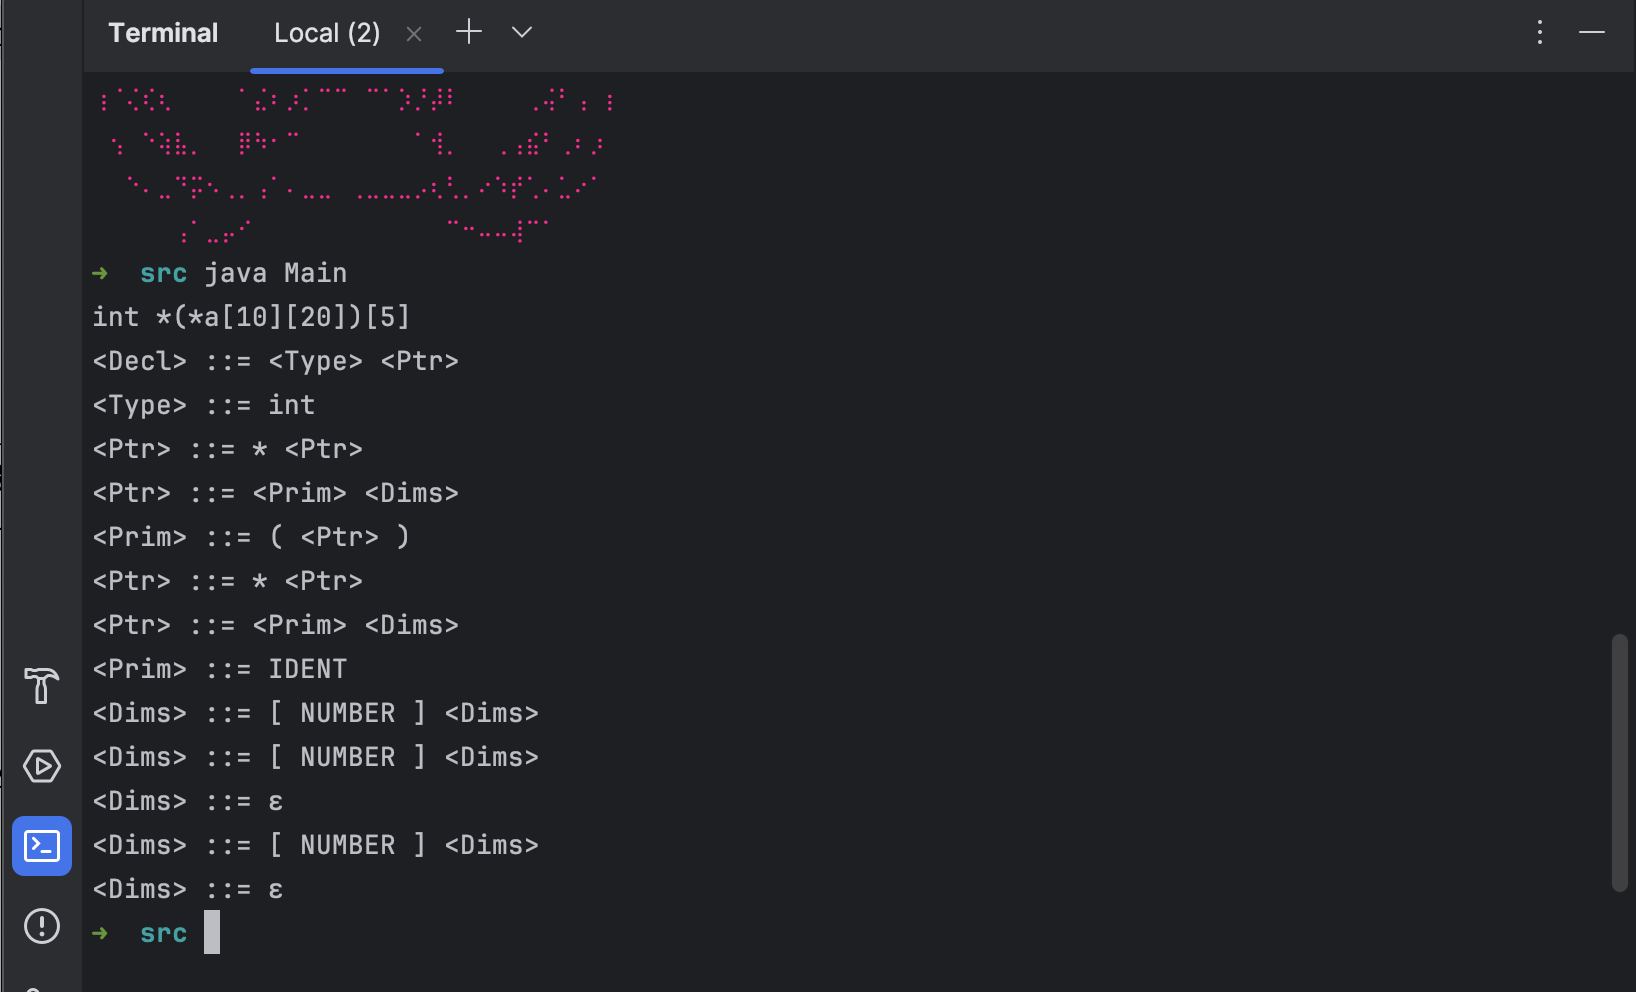
\includegraphics[width=0.8\textwidth]{фото18.jpeg}
    \captionof{figure}{вывод}
\end{center}
\newpage
\section{Вывод}
В ходе выполнения лабораторной работы были получены навыки разработки синтаксического анализатора для языка C-подобных объявлений указателей и массивов. Написана программа, которая корректно разбирает конструкции вида int *(*a[10][20])[5] и выводит последовательность применённых правил грамматики.

Основные результаты:

Освоен принцип работы LL(1-грамматик и рекурсивного спуска.

Реализован обработчик ошибок с точным указанием позиции в тексте.

Программа успешно анализирует корректные объявления и детектирует синтаксические ошибки.

Работа позволила лучше понять устройство компиляторов и этапы синтаксического разбора.

\end{document}